\documentclass{article}\usepackage[]{graphicx}\usepackage[]{color}
%% maxwidth is the original width if it is less than linewidth
%% otherwise use linewidth (to make sure the graphics do not exceed the margin)
\makeatletter
\def\maxwidth{ %
  \ifdim\Gin@nat@width>\linewidth
    \linewidth
  \else
    \Gin@nat@width
  \fi
}
\makeatother

\definecolor{fgcolor}{rgb}{0.345, 0.345, 0.345}
\newcommand{\hlnum}[1]{\textcolor[rgb]{0.686,0.059,0.569}{#1}}%
\newcommand{\hlstr}[1]{\textcolor[rgb]{0.192,0.494,0.8}{#1}}%
\newcommand{\hlcom}[1]{\textcolor[rgb]{0.678,0.584,0.686}{\textit{#1}}}%
\newcommand{\hlopt}[1]{\textcolor[rgb]{0,0,0}{#1}}%
\newcommand{\hlstd}[1]{\textcolor[rgb]{0.345,0.345,0.345}{#1}}%
\newcommand{\hlkwa}[1]{\textcolor[rgb]{0.161,0.373,0.58}{\textbf{#1}}}%
\newcommand{\hlkwb}[1]{\textcolor[rgb]{0.69,0.353,0.396}{#1}}%
\newcommand{\hlkwc}[1]{\textcolor[rgb]{0.333,0.667,0.333}{#1}}%
\newcommand{\hlkwd}[1]{\textcolor[rgb]{0.737,0.353,0.396}{\textbf{#1}}}%

\usepackage{framed}
\makeatletter
\newenvironment{kframe}{%
 \def\at@end@of@kframe{}%
 \ifinner\ifhmode%
  \def\at@end@of@kframe{\end{minipage}}%
  \begin{minipage}{\columnwidth}%
 \fi\fi%
 \def\FrameCommand##1{\hskip\@totalleftmargin \hskip-\fboxsep
 \colorbox{shadecolor}{##1}\hskip-\fboxsep
     % There is no \\@totalrightmargin, so:
     \hskip-\linewidth \hskip-\@totalleftmargin \hskip\columnwidth}%
 \MakeFramed {\advance\hsize-\width
   \@totalleftmargin\z@ \linewidth\hsize
   \@setminipage}}%
 {\par\unskip\endMakeFramed%
 \at@end@of@kframe}
\makeatother

\definecolor{shadecolor}{rgb}{.97, .97, .97}
\definecolor{messagecolor}{rgb}{0, 0, 0}
\definecolor{warningcolor}{rgb}{1, 0, 1}
\definecolor{errorcolor}{rgb}{1, 0, 0}
\newenvironment{knitrout}{}{} % an empty environment to be redefined in TeX

\usepackage{alltt}
\usepackage[sc]{mathpazo}
\usepackage[T1]{fontenc}
\usepackage{geometry}
\geometry{verbose,tmargin=2.5cm,bmargin=2.5cm,lmargin=2.5cm,rmargin=2.5cm}
\setcounter{secnumdepth}{2}
\setcounter{tocdepth}{2}
\usepackage{url}
\usepackage[unicode=true,pdfusetitle,
 bookmarks=true,bookmarksnumbered=true,bookmarksopen=true,bookmarksopenlevel=2,
 breaklinks=false,pdfborder={0 0 1},backref=false,colorlinks=false]
 {hyperref}
\hypersetup{
 pdfstartview={XYZ null null 1}}
\usepackage{breakurl}
\IfFileExists{upquote.sty}{\usepackage{upquote}}{}
\begin{document}





\title{A Minimal Demo of knitr}


\author{Yihui Xie}

\maketitle
You can test if \textbf{knitr} works with this minimal demo. OK, let's
get started with some boring random numbers:

\begin{knitrout}
\definecolor{shadecolor}{rgb}{0.969, 0.969, 0.969}\color{fgcolor}\begin{kframe}
\begin{alltt}
\hlkwd{set.seed}\hlstd{(}\hlnum{1121}\hlstd{)}
\hlstd{(x} \hlkwb{<-} \hlkwd{rnorm}\hlstd{(}\hlnum{20}\hlstd{))}
\end{alltt}
\begin{verbatim}
##  [1]  0.14496  0.43832  0.15319  1.08494  1.99954 -0.81188  0.16027  0.58589  0.36009
## [10] -0.02531  0.15088  0.11008  1.35968 -0.32699 -0.71638  1.80977  0.50840 -0.52746
## [19]  0.13272 -0.15594
\end{verbatim}
\begin{alltt}
\hlkwd{mean}\hlstd{(x)}
\end{alltt}
\begin{verbatim}
## [1] 0.3217
\end{verbatim}
\begin{alltt}
\hlkwd{var}\hlstd{(x)}
\end{alltt}
\begin{verbatim}
## [1] 0.5715
\end{verbatim}
\end{kframe}
\end{knitrout}


The first element of \texttt{x} is 0.145. Boring boxplots
and histograms recorded by the PDF device:

\begin{knitrout}
\definecolor{shadecolor}{rgb}{0.969, 0.969, 0.969}\color{fgcolor}\begin{kframe}
\begin{alltt}
\hlcom{## two plots side by side (option fig.show='hold')}
\hlkwd{par}\hlstd{(}\hlkwc{mar} \hlstd{=} \hlkwd{c}\hlstd{(}\hlnum{4}\hlstd{,} \hlnum{4}\hlstd{,} \hlnum{0.1}\hlstd{,} \hlnum{0.1}\hlstd{),} \hlkwc{cex.lab} \hlstd{=} \hlnum{0.95}\hlstd{,} \hlkwc{cex.axis} \hlstd{=} \hlnum{0.9}\hlstd{,} \hlkwc{mgp} \hlstd{=} \hlkwd{c}\hlstd{(}\hlnum{2}\hlstd{,} \hlnum{0.7}\hlstd{,} \hlnum{0}\hlstd{),} \hlkwc{tcl} \hlstd{=} \hlopt{-}\hlnum{0.3}\hlstd{,}
    \hlkwc{las} \hlstd{=} \hlnum{1}\hlstd{)}
\hlkwd{boxplot}\hlstd{(x)}
\hlkwd{hist}\hlstd{(x,} \hlkwc{main} \hlstd{=} \hlstr{""}\hlstd{)}
\end{alltt}
\end{kframe}

{\centering 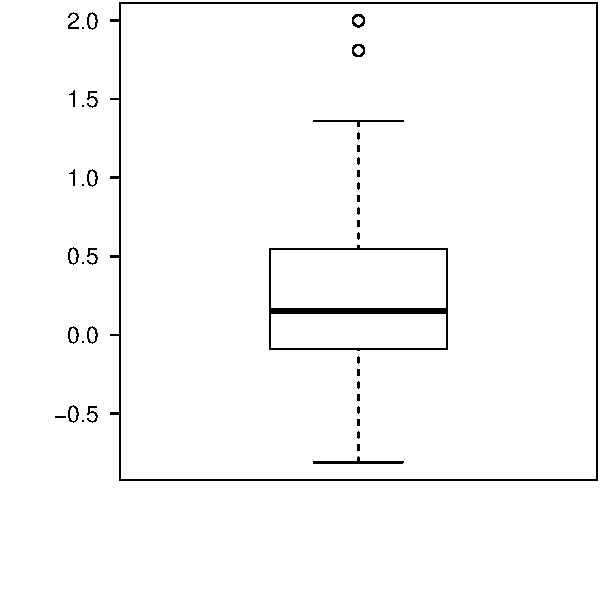
\includegraphics[width=.4\linewidth]{figure/minimal-boring-plots1} 
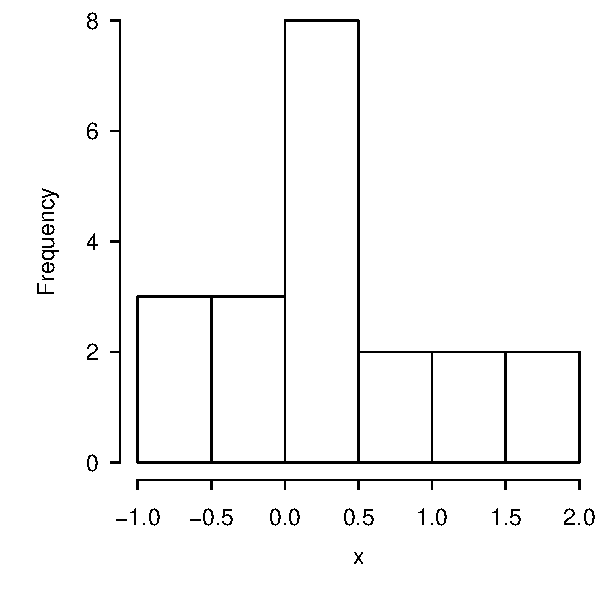
\includegraphics[width=.4\linewidth]{figure/minimal-boring-plots2} 

}



\end{knitrout}

Do the above chunks work? You should be able to compile the \TeX{}
document and get a PDF file like this one: \url{https://bitbucket.org/stat/knitr/downloads/knitr-minimal.pdf}.
The Rnw source of this document is at \url{https://github.com/yihui/knitr/blob/master/inst/examples/knitr-minimal.Rnw}.

\end{document}
